\documentclass[border=4pt]{standalone}
\usepackage{tikz}
\usetikzlibrary{arrows.meta,positioning,fit,backgrounds,calc,shapes.geometric}
\definecolor{snblue}{HTML}{1F5A96}
\definecolor{snred}{HTML}{B8433A}
\definecolor{sngreen}{HTML}{3A8A4A}
\tikzset{
  pb/.style={rectangle,rounded corners=3pt,draw=snblue!60,fill=snblue!8,text width=2.3cm,align=center,inner sep=4pt,line width=0.5pt,font=\small},
  db/.style={pb,draw=snred!55,fill=snred!6},
  gb/.style={pb,draw=sngreen!60,fill=sngreen!8},
  dm/.style={diamond,aspect=2.2,draw=gray!70,fill=gray!6,align=center,inner sep=1pt,font=\small},
  ar/.style={-Stealth,line width=0.6pt,gray!70}}

\begin{document}
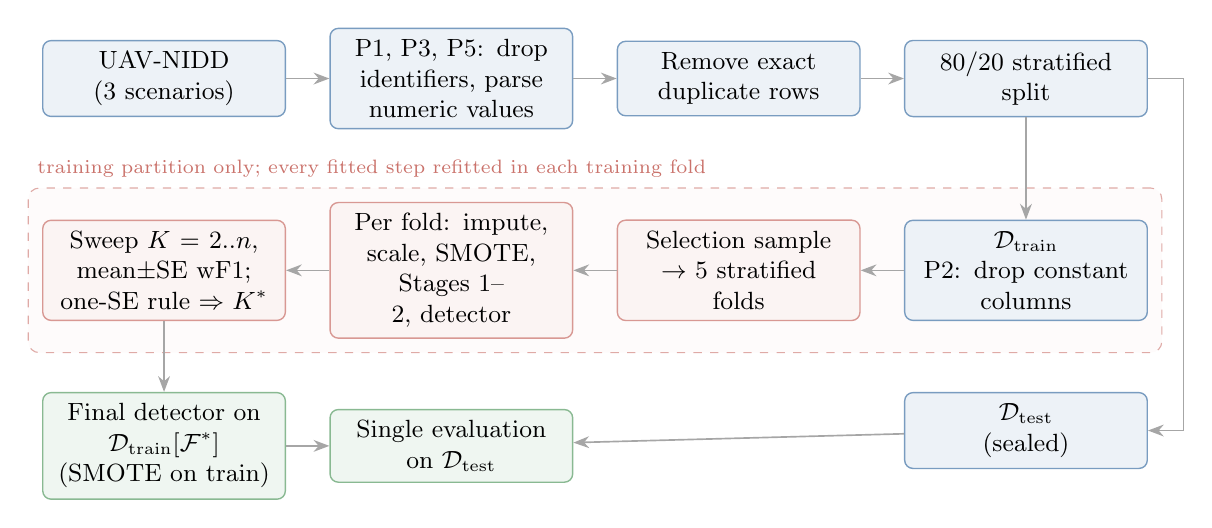
\begin{tikzpicture}[node distance=0.5cm and 0.55cm,pb/.append style={text width=2.8cm}]
% row 1 (left to right)
\node[pb](raw){UAV-NIDD\\(3 scenarios)};
\node[pb,right=of raw](pre){P1, P3, P5: drop\\identifiers, parse\\numeric values};
\node[pb,right=of pre](dd){Remove exact\\duplicate rows};
\node[pb,right=of dd](sp){80/20 stratified\\split};
% row 2 (right to left): training partition only
\node[pb,below=1.3cm of sp](tr){$\mathcal{D}_{\mathrm{train}}$\\P2: drop constant\\columns};
\node[db,left=of tr](ss){Selection sample\\$\to$ 5 stratified\\folds};
\node[db,left=of ss](fo){Per fold: impute,\\scale, SMOTE,\\Stages 1--2, detector};
\node[db,left=of fo](sw){Sweep $K=2..n$,\\mean$\pm$SE wF1;\\one-SE rule $\Rightarrow K^{*}$};
% row 3 (left to right)
\node[gb,below=0.9cm of sw](fin){Final detector on\\$\mathcal{D}_{\mathrm{train}}[\mathcal{F}^{*}]$\\(SMOTE on train)};
\node[gb,right=of fin](ev){Single evaluation\\on $\mathcal{D}_{\mathrm{test}}$};
\node[pb,below=0.9cm of tr](te){$\mathcal{D}_{\mathrm{test}}$\\(sealed)};
\begin{scope}[on background layer]
\node[draw=snred!45,dashed,rounded corners=4pt,fill=snred!2,inner sep=5pt,fit=(tr)(ss)(fo)(sw)](box){};
\end{scope}
\node[font=\scriptsize,text=snred!75,anchor=south west,text width=12cm] at (box.north west){training partition only; every fitted step refitted in each training fold};
\draw[ar](raw)--(pre);\draw[ar](pre)--(dd);\draw[ar](dd)--(sp);
\draw[ar](sp)--(tr);\draw[ar](tr)--(ss);\draw[ar](ss)--(fo);\draw[ar](fo)--(sw);
\draw[ar](sw)--(fin);\draw[ar](fin)--(ev);\draw[ar](te)--(ev);
\draw[ar](sp.east)--++(0.45,0)|-(te.east);
\end{tikzpicture}
\end{document}
